\documentclass{sikslides}

\usepackage{bm}
\usepackage{tabu}
\tabulinesep=1.2mm
\usepackage{subcaption}
\usepackage{graphicx}

\newcommand*{\vcenterimage}[2]{\vcenter{\hbox{\includegraphics[height=#1]{#2}}}}
\newcommand*{\vcenterarrow}{\vcenter{\hbox{$\bm{\Longrightarrow}$}}}

\title[Security Considerations for CPS]{Security Considerations for Cyber-Physical Systems}
\subtitle{Seminar \\Cyber-Physical Systems} % Bachelor
\author{Maximilian Ammann}
\date[01.02.2019]{01. Februar 2019}
\setbeamercovered{invisible}
\setbeamertemplate{section in toc}[sections numbered]
\setbeamertemplate{subsection in toc}[subsections numbered]
\begin{document}

    \titleframe

    \begin{frame}
        \frametitle{Unterschied von Cybersecurity und Cyber-physical Security}
        \centering
        \only<1>{
            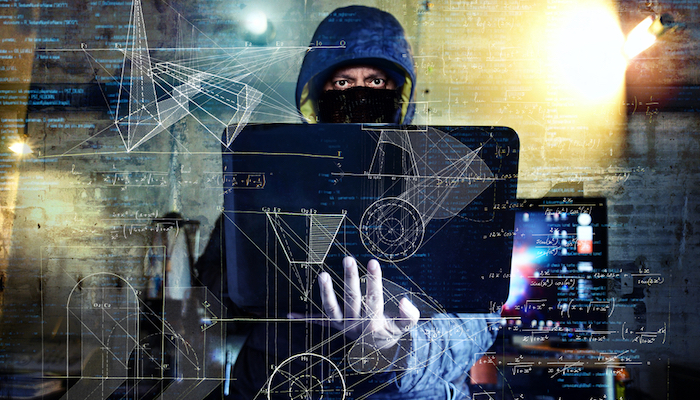
\includegraphics[height=6cm]{figure/hacker.jpg}
        }

        \only<2>{
            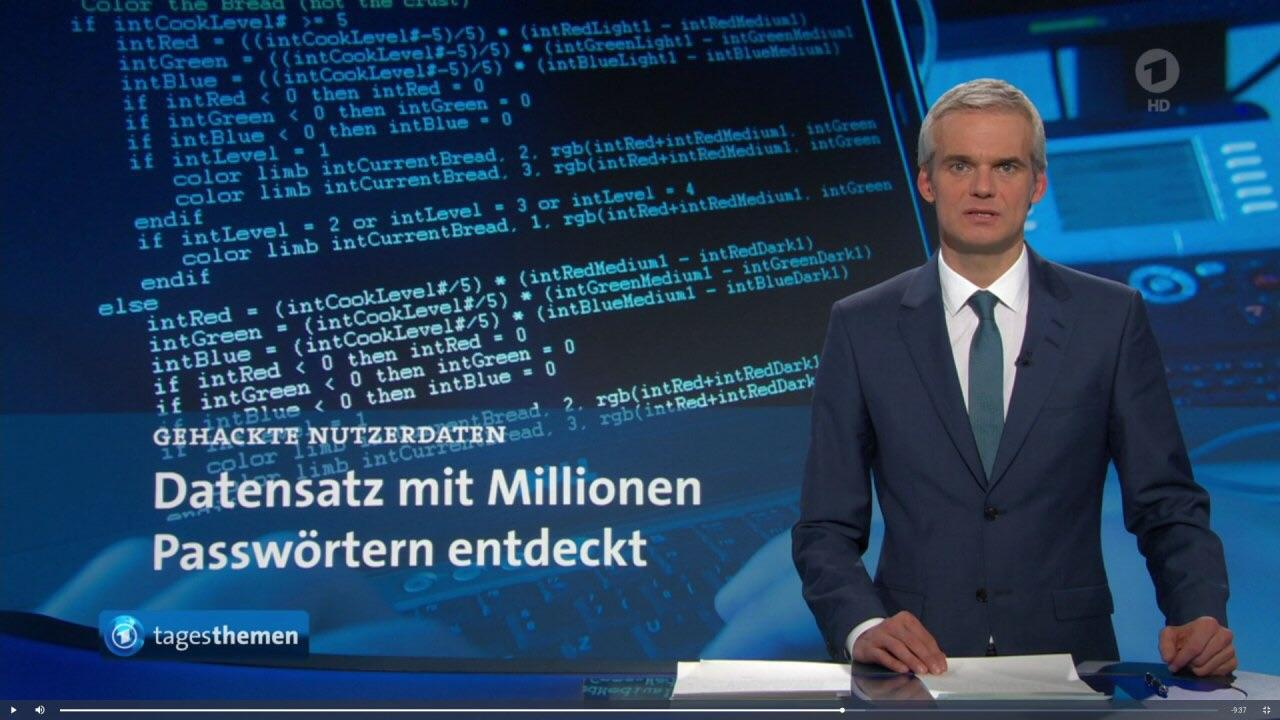
\includegraphics[height=6cm]{figure/cyberattack.jpg}
            \hspace*{10pt}\hbox{\scriptsize Quelle:\thinspace{\scriptsize\itshape Tagesschau 17.01.2019}}
        }

        \pause
        \vspace{4mm}
        \textbf{Cybersecurity $\neq$ Cyber-physical Security}

        \textbf{Security $\neq$ Safety}
    \end{frame}

    \begin{frame}
        \frametitle{Gliederung}
        \tableofcontents[hideallsubsections,pausesections]
        %\tableofcontents[pausesections]
        %\tableofcontents
    \end{frame}

    %    \sectionframe{Eigenschaften von CPS und Angriffsszenarios}
    \section{Eigenschaften von CPS und Angriffsszenarios}

    \begin{frame}[label=abstrakt]
        \frametitle{Abstraktion eines Cyber-physical Systems}
        \begin{figure}
            \centering
            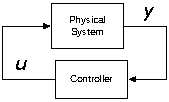
\includegraphics[width=5cm]{../figure/abstrakt}
        \end{figure}
    \end{frame}

    \begin{frame}
        \frametitle{Von CIA-Dreieck zu CIAANV-Hexagon?!}
        \centering
        $\vcenterimage{2.5cm}{../figure/cia}\vcenterarrow\vcenterimage{3.5cm}{../figure/triad}$

        \vspace{40px}
        $\rightarrow$ Komplexere Situation durch erweiterte Angriffsfläche bei CPS
    \end{frame}

    \begin{frame}
        <1>[label=eigenschaften]
        \frametitle{Eigenschaften}

        \begin{overlayarea}{\textwidth}{10cm}
        \begin{tabu}
            to \linewidth { | X[1.6,l] | X[5,l] | }
            \hline
            Eigenschaft: $e$&Ein System hat Eigenschaft $e$ genau dann, wenn~\ldots \\
            \hline
            \only<1>{\bf}
            Availability&
            \only<1>{\bf}
            \ldots Ressourcen für autorisierte Teilnehmer angemessen verfügbar ist. \\
            \hline
            \only<2>{\bf}
            \uncover<2->{Confidentiality}&
            \only<2>{\bf}
            \uncover<2->{\ldots nur autorisierte Teilnehmer auf Ressourcen zugreifen können.}\\
            \hline
            \only<3>{\bf}
            \uncover<3->{Integrity}&
            \only<3>{\bf}
            \uncover<3->{\ldots Ressourcen nur von autorisierten Teilnehmern verändert werden können.} \\
            \hline
            \only<4>{\bf}
            \uncover<4->{Authenticity}&
            \only<4>{\bf}
            \uncover<4->{\ldots sich beide Kommunikationspartner einig über die Identität des Gegenübers sind.} \\
            \hline
            \only<5>{\bf}
            \uncover<5>{Veracity und Plausibility} &
            \only<5>{\bf}
            \uncover<5>{\ldots Aussagen des Systems der Wahrhaftigkeit der Wirklichkeit entsprechen.} \\
            \hline
            %Non-repudiation &
            %\ldots jedes Ereignis, welches das System beeinflusst, nachvollzogen werden kann. \\
            %\hline
        \end{tabu}
\end{overlayarea}
    \end{frame}

    \subsection{Denial-of-Service Angriff}
    \begin{frame}
        \frametitle{Szenario: Denial-of-Service Angriff}
        \begin{figure}
            \centering
            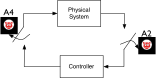
\includegraphics[width=4cm]{figure/dos}
            % \caption{Abstraktion eines DoS Angriffs}
        \end{figure}
        \begin{itemize}
            \item Ziel: Mit großer Flut an Informationen die \textbf{Availability} des CPS stören
            \pause
            \item Beispiele:
            \begin{itemize}
                \item CAN Busse in Autos: Fehlfunktion der Warnlichter, Diebstahlsicherung
                \item Echtzeitkritische Stromnetze: Störung des Normalbetrieb
            \end{itemize}
            \pause
            \item Bei mehreren Angreifern: Distributed-DoS
            \item Kabellose Kommunikation meist anfälliger wegen geringer Bandbreite
        \end{itemize}
    \end{frame}

    \subsection{Man-in-the-Middle Angriff}
    % Continue to Confidentiality, Integrity, Authenticity
    \againframe<2>{eigenschaften}
    \againframe<3>{eigenschaften}
    \againframe<4>{eigenschaften}

    \begin{frame}[t]
        \frametitle{Szenario: Man-in-the-Middle Angriff}
        \begin{overlayarea}{\linewidth}{4cm}
        \begin{figure}
            \centering
            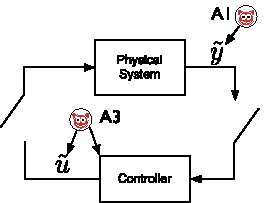
\includegraphics[width=4cm]{figure/mitm}
            % \caption{Abstraktion eines MITM Angriffs}
        \end{figure}
        \end{overlayarea}
        \begin{onlyenv}<1-2>
            \begin{itemize}
                \item Passiv: Nur lauschen
                \begin{itemize}
                    \item Verletzung der \textbf{Confidentiality} des CPS
                    \pause
                \end{itemize}
                \item Aktiv: Verändern der Daten
                \begin{itemize}
                    \item Bei fehlender \textbf{Authenticity}: Keine Verifikation der Identität möglich
                    \item Bei fehlender \textbf{Integrity}: Keine überprüfung auf Veränderung der Daten (Prüfsummen!)
                \end{itemize}
                \pause
            \end{itemize}
        \end{onlyenv}

        \begin{onlyenv}<3-4>
            \begin{itemize}
                \item Beispiele:
                \begin{itemize}
                    \item ARP-Poisoning in IEE 802.11 und Local Area Networks
                    \pause
                    \item Offline Replay Angriffe bei Autos
                \end{itemize}
            \end{itemize}
        \end{onlyenv}

    \end{frame}

    \subsection{Angriff auf das physische System}
    % Continue to Veracity
    \againframe<5>{eigenschaften}
    \begin{frame}
        \frametitle{Szenario: Angriff auf das physische System}
        \begin{figure}
            \centering
            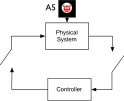
\includegraphics[width=4cm]{figure/physical}
            % \caption{Abstraktion eines physischen Angriffs}
        \end{figure}
        \begin{itemize}
            \item Ziel: Verändern der Daten bevor diese an das Cybersystem geschickt werden
            \item Authenticity hilft nicht \textbf{Veracity} sicherzustellen
            \pause
            \item Beispiele:
            \begin{itemize}
                \item Manipulation von physischen Prozessen führt zu Wechselwirkungen
                \item Manipulation von Sensoren
            \end{itemize}
        \end{itemize}
    \end{frame}

    % Continue to Non-repudiation
    % \againframe<6>{eigenschaften}

    \bgroup
    \setbeamercolor{background canvas}{bg=black}
    \begin{frame}[plain]{}
        \centering
        \Huge\textbf{\textcolor{white}{Time to zoom out!}}
    \end{frame}
    \egroup

    \sectionframe{Proaktive Maßnahmen: Verhindern von Angriffen}
    \begin{frame}[t]
        \frametitle{Proaktive Maßnahmen: Verhindern von Angriffen}
        \begin{overlayarea}{\linewidth}{1cm}
            \begin{block}{}
                Proaktive Maßnahmen: Maßnahmen, die vor dem Angriff getroffen werden müssen
            \end{block}
        \end{overlayarea}

        \vspace{2cm}

        \begin{onlyenv}<1-3>
            \begin{itemize}[<+->]
                \item Authentisierung der Kommunikationspartner durch z.B. Signaturen $\rightarrow$ \textbf{Authenticity}
                \item Verschlüsselung der Kommunikationsdaten $\rightarrow$ \textbf{Confidentiality}
                \item Prüfsummen zur Validierung der Kommunikation $\rightarrow$ \textbf{Integrity}
            \end{itemize}

        \end{onlyenv}


        \begin{onlyenv}<4-7>
            \begin{itemize}[<+->]
                \item Transportverschlüsselung: TLS für TCP, DTLS für UDP, Logicial Link Transport Protocol für NFC $\rightarrow$ \textbf{Confidentiality, Integrity, Authenticity}
                \item Redundanzen und Diversität für CPS $\rightarrow$ \textbf{Availability}
                \item Hardware Security Module: Verhindern Auslesen von Secrets wie Schlüssel
                \item Verifikation von Programmen: Reduzieren von Lücken durch z.B.\ Code-Audits oder Fuzzing
            \end{itemize}
        \end{onlyenv}

        \begin{onlyenv}<8>
            \begin{itemize}
                \item Trennung von Netzwerken
                \item Trennung von Privilegien
                \item Least Privilege-Prinzip
                \pause
            \end{itemize}
        \end{onlyenv}

        \begin{onlyenv}<9>
            \begin{itemize}
                \item Abschreckung durch Gesetze
                \item Physische Baumaßnahmen (Allerdings ist ein Cyberangriff sehr viel Wahrscheinlicher)
            \end{itemize}
        \end{onlyenv}
    \end{frame}

    \sectionframe{Reaktive Maßnahmen: Detektion und Wiederherstellung}
    \begin{frame}
        \frametitle{Reaktive Maßnahmen: Detektion und Wiederherstellung}
        \begin{block}{}
            Reaktive Maßnahmen: Maßnahmen, die auf Angriffe reagieren
        \end{block}
        \begin{itemize}
            \item Beispiele:
            \begin{itemize}
                \item Überwachung von Sensoren eines Kraftwerkes $\rightarrow$ \textbf{Veracity}
                \item Wiederherstellung der physischen und Cybersystemen mithilfe von Checkpoints $\rightarrow$ \textbf{Veracity}
            \end{itemize}
        \end{itemize}
    \end{frame}

    \begin{frame}
        \frametitle{Überwachung von Sensoren}
        \begin{figure}
            \centering
            \begin{subfigure}{0.49\textwidth}
                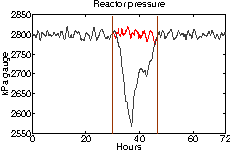
\includegraphics[height=3cm]{../figure/entropy_a}
                \caption{Gefälschte Werte eines Sensors}
            \end{subfigure}
            \begin{subfigure}{0.49\textwidth}
                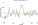
\includegraphics[height=3cm]{../figure/entropy_b}
                \caption{Entropie des gesamten Kraftwerks}
            \end{subfigure}
        \end{figure}
    \end{frame}

    \begin{frame}
        \frametitle{Fazit}

        \begin{center}
               \bf Sicherheit für CPS bedarf spezieller Betrachtung
        \end{center}

        \begin{itemize}
            \item Angriffsvektoren sind andere als bei klassischen Cybersystemen
            \item Man muss CPS oft mehr vertrauen entgegenbringen als Cybersystemen
        \end{itemize}
    \end{frame}
\end{document}

